\documentclass[12pt]{article}

\usepackage{amsmath}
\usepackage{graphicx}
\usepackage{dcolumn}
\usepackage{booktabs}
\usepackage{rotating}
\usepackage{subcaption}
\usepackage{listings}

\usepackage{setspace}
\usepackage{parskip}
\usepackage[top=1in,bottom=1in,left=1in,right=1in]{geometry}

\usepackage{natbib}
\usepackage[pdfstartpage=1,pdfpagemode=UseNone,pdfstartview=FitH,pdffitwindow=true,bookmarks=false,colorlinks=true,linkcolor=blue,citecolor=blue]{hyperref}

% define lightgray
\usepackage[table]{xcolor}
\definecolor{lightgray}{gray}{0.9}

\begin{document}


%%%%%%%%%%%%%%%%%%%%%%%%%%%%%%%%
% Tables
%%%%%%%%%%%%%%%%%%%%%%%%%%%%%%%%
{\bf Title:} Tuning DataSynthesizer \\
{\bf Authors:} Jonathan P. Latner \\
{\bf Revision date:} \today

\section{DataSynthesizer hyperparameters}

\url{https://github.com/DataResponsibly/DataSynthesizer/blob/master/notebooks/DataSynthesizer__correlated_attribute_mode.ipynb}


\begin{itemize}
    \item Total 63 combinations of tuning parameters (336 synthetic data sets)
    \item k (3: 0, 1, 2).  The maximum number of parents in Bayesian network, i.e., the maximum number of incoming edges.  Default is 0.
    \item epsilon (7: 0, 0.1, 1, 5, 10, 20, 30).  It roughly means that removing a row in the input dataset will not change the probability of getting the same output more than a multiplicative difference of exp(epsilon).  Increase epsilon value to reduce the injected noises. Set epsilon=0 to turn off differential privacy.  Default is 0.1.
    \item copies (3: 1, 5, 10): Number of synthetic data sets
\end{itemize}

\section{Utility parameters}

Following previous work, the utility of the synthetic and sample data was assessed using multiple measures. The confidence interval overlap (CIO) and ratio of counts/estimates (ROC) were calculated. This was to provide a more complete picture of the utility, rather than relying upon just one measure. The propensity score mean squared error (pMSE) was not used as, whilst it is suitable for analysing the synthetic data it is not suited to the analysis of sample data as it is structurally tied to the original data (since the sample data is a subset of the original data).

ROE is calculated by taking the ratio of the synthetic and original data estimates, where the smaller of these two estimates is divided by the larger one. Thus, given two corresponding estimates (e.g. totals, proportions), where $y^1_{orig}$ is the estimate orig from the original data and $y^1_{synth}$ is the corresponding estimate from the synthetic synth data, the ROE is calculated as:

\begin{equation}
    ROE = \frac{min(y^1_{orig},y^1_{synth})}{max(y^1_{orig},y^1_{synth})}
\end{equation}

If $y^1_{orig}$ = $y^1_{synth}$, then ROE = 1.  The ROE will be calculated over bivariate and univariate data, and takes a value between 0 and 1. For each categorical variable the ratio of estimates are averaged across categories to give an overall ratio of estimates.

To calculate the CIO (using 95\% confidence intervals), the coefficients from regression models built on the original and synthetic datasets are used. The CIO, proposed by Karr et al. [17], is defined as:

\begin{equation}
    CIO = \frac{1}{2}\left\{\frac{min(\mu_o,\mu_s)-max(l_o,l_s)}{\mu_o - l_o} + \frac{min(\mu_o,\mu_s)-max(l_o,l_s)}{\mu_s - l_s}\right\}
\end{equation}

where $\mu_o, l_o, l_s$ denote the respective upper and lower bounds of the confidence intervals for the original and synthetic data. This can be summarised by the average across all regression coefficients, with a higher CIO indicating greater utility (maximum value is 1 and a negative value indicating no overlap).  Here, categorical variables are modified so that within each variable the maximum value within each variable is 1 and all other values are coded as 0.  We use linear probability models to compare across variables.  Each variable in the data set is a dependent variable and all other variables are independent variables, respectively.

\clearpage
\section{Graphs}

\begin{figure}[!h]
    \centering
    \caption{Frequency of counts}
    \resizebox{\textwidth}{!}{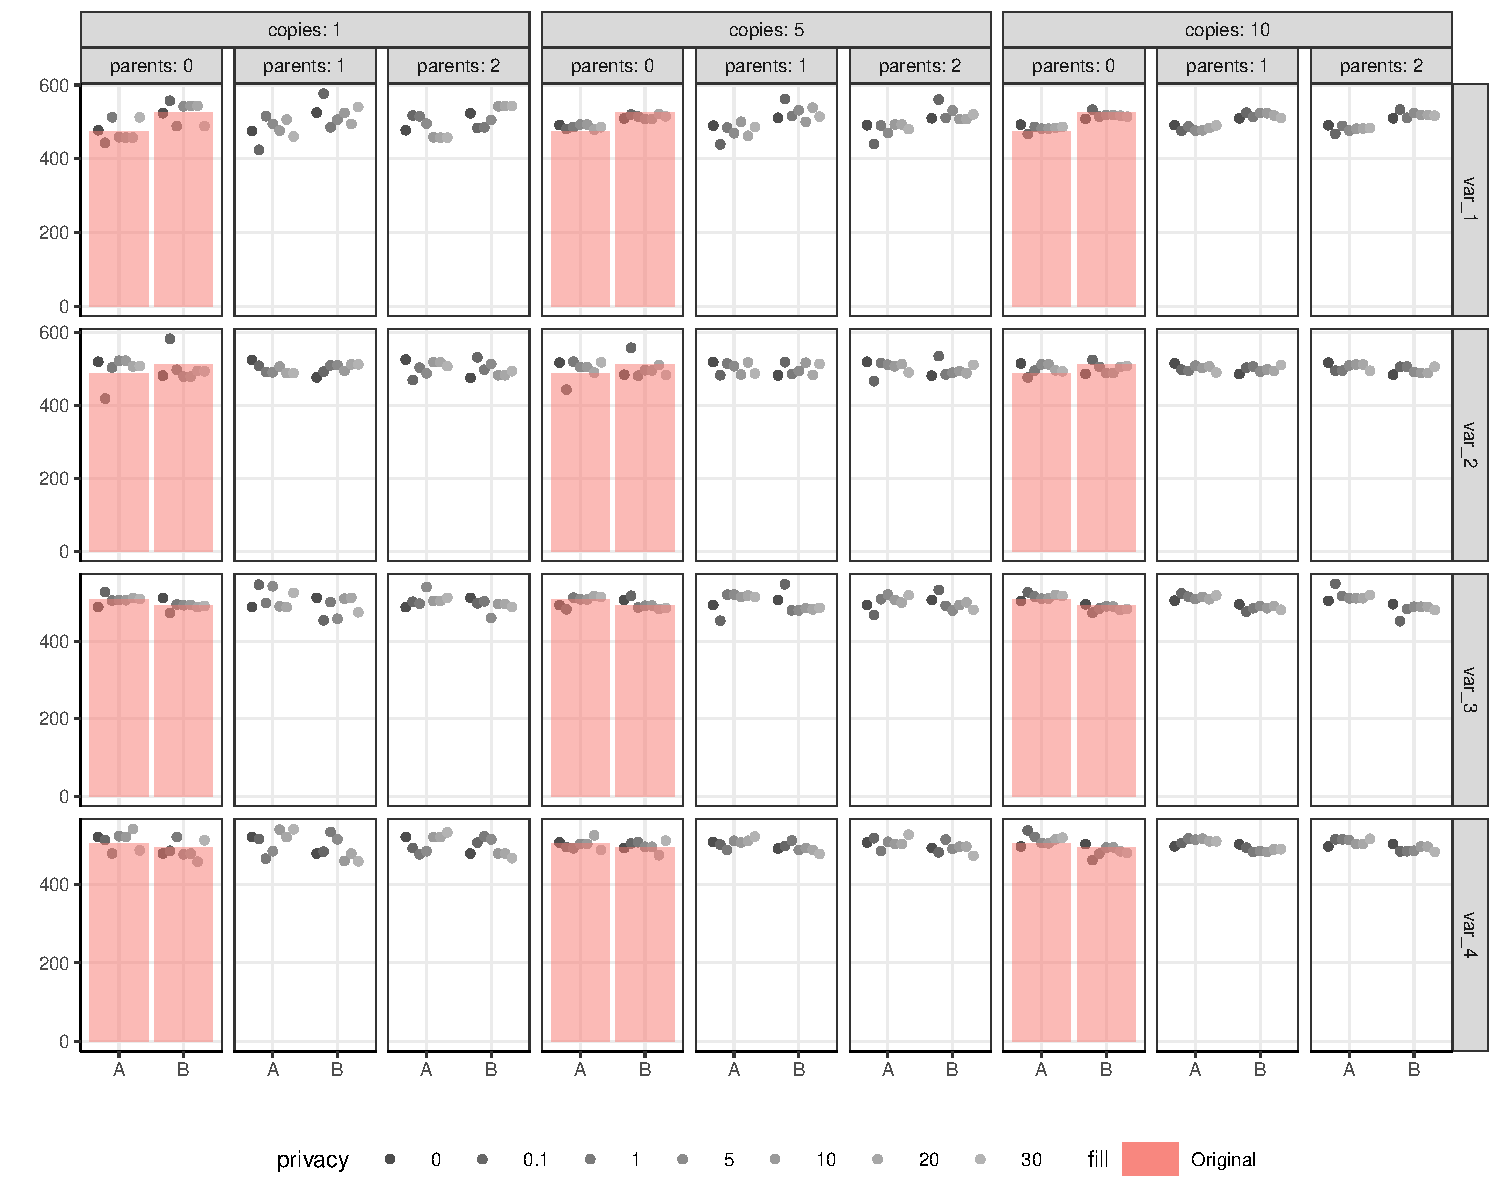
\includegraphics{../graphs/datasynthesizer/graph_datasynthesizer_frequency.pdf}}
    \label{graph_datasynthesizer_frequency}
\end{figure}

\begin{figure}[!h]
    \centering
    \caption{Ratio of estimates (ROE) - univariate}
    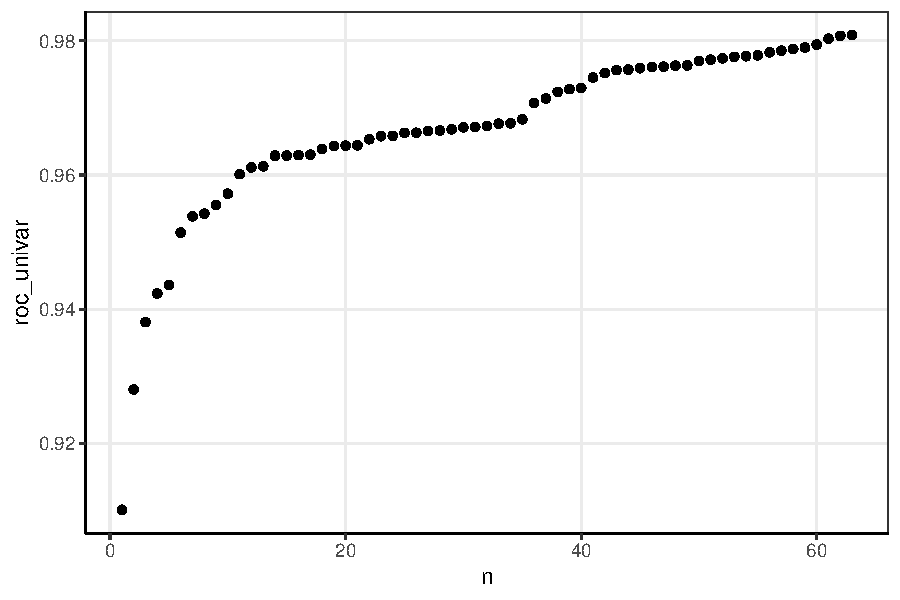
\includegraphics{../graphs/datasynthesizer/graph_datasynthesizer_roc_univar_raw.pdf}
    \label{graph_datasynthesizer_roc_univar_raw}
\end{figure}

\begin{figure}[!h]
    \centering
    \caption{Parametric estimates of tuning parameters on ROE}
    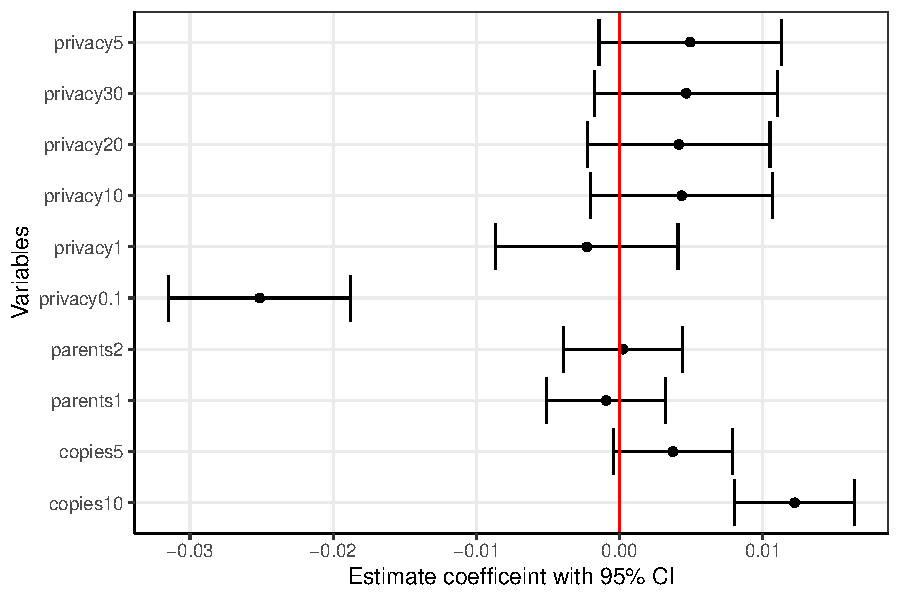
\includegraphics{../graphs/datasynthesizer/graph_datasynthesizer_roc_univar.pdf}
    \label{graph_datasynthesizer_roc_univar}
\end{figure}

\begin{figure}[!h]
    \centering
    \caption{Parametric estimates of tuning parameters on ROE by copies (m)}
    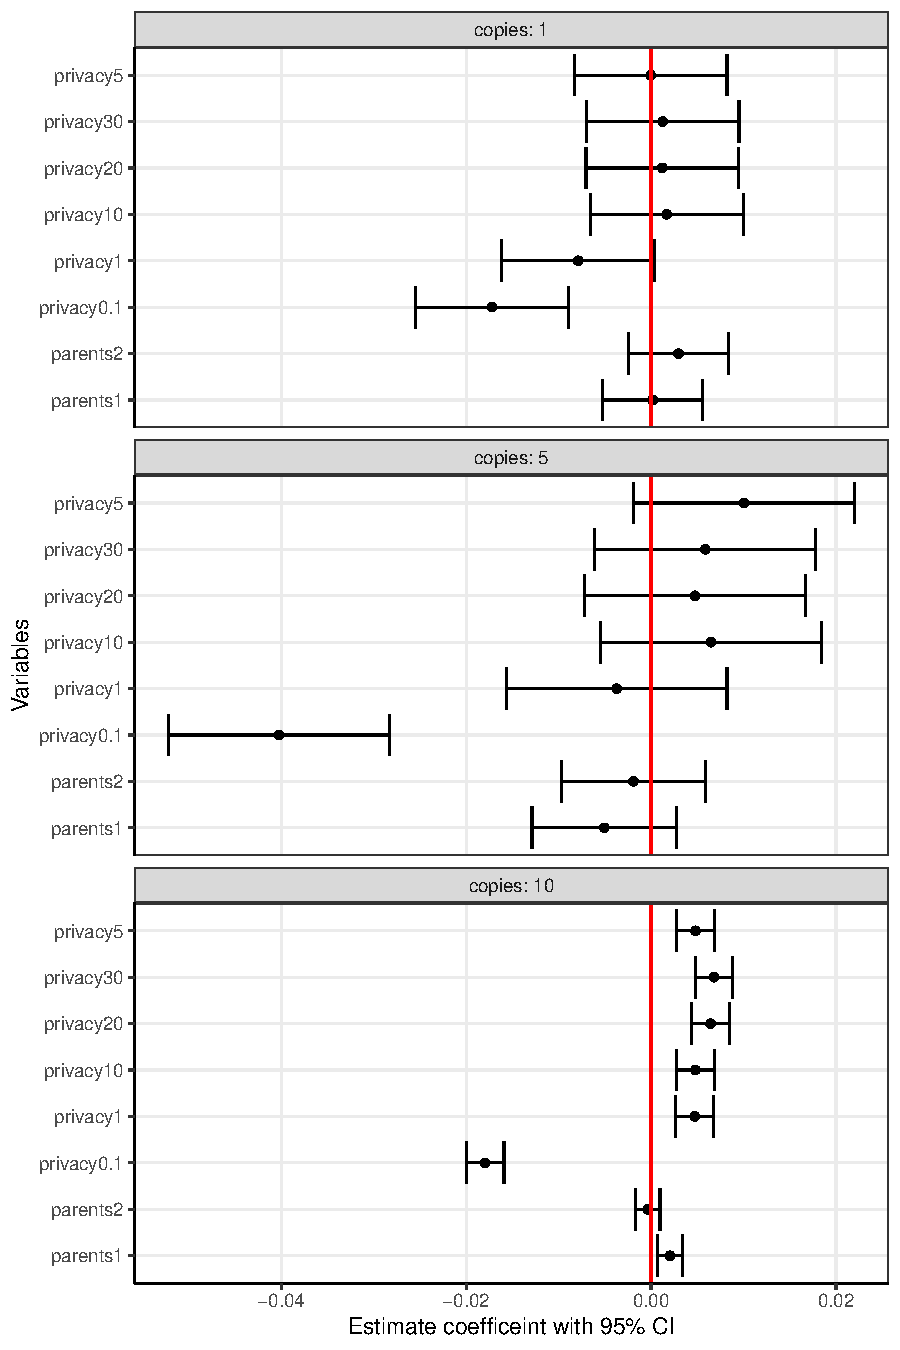
\includegraphics{../graphs/datasynthesizer/graph_datasynthesizer_roc_univar_facet.pdf}
    \label{graph_datasynthesizer_roc_univar_facet}
\end{figure}

\begin{figure}[!h]
    \centering
    \caption{Ratio of estimates - confidence interval overlap (CIO)}
    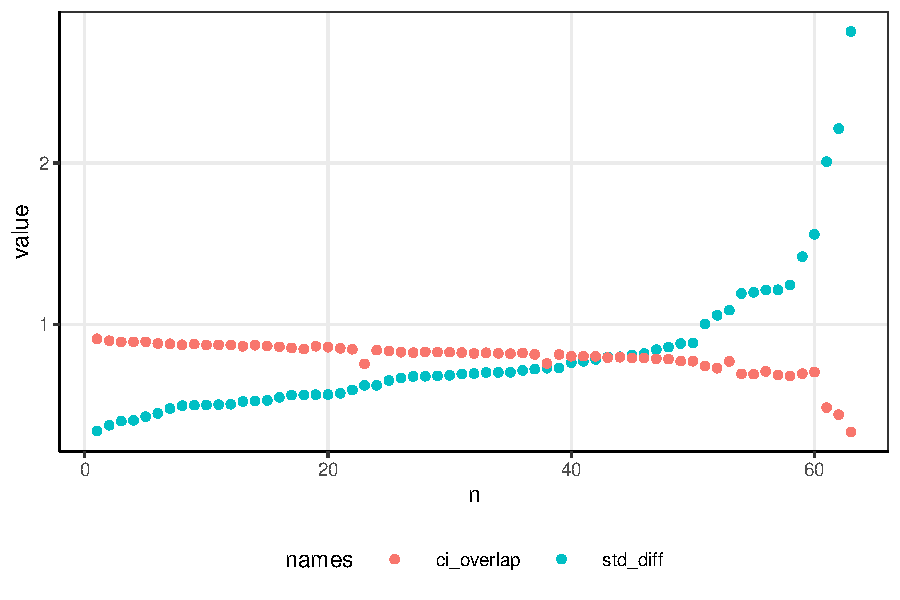
\includegraphics{../graphs/datasynthesizer/graph_datasynthesizer_cio_raw.pdf}
    \label{graph_datasynthesizer_cio}
\end{figure}

\begin{figure}[!h]
    \centering
    \caption{Parametric estimates of tuning parameters on CIO}
    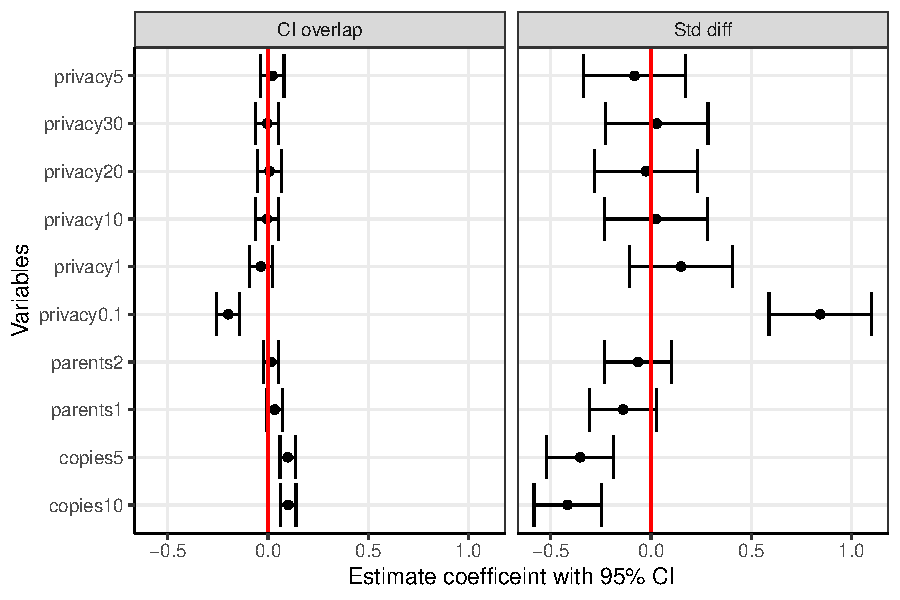
\includegraphics{../graphs/datasynthesizer/graph_datasynthesizer_cio.pdf}
    \label{graph_datasynthesizer_cio}
\end{figure}

\begin{figure}[!h]
    \centering
    \caption{Parametric estimates of tuning parameters on CIO by copies (m)}
    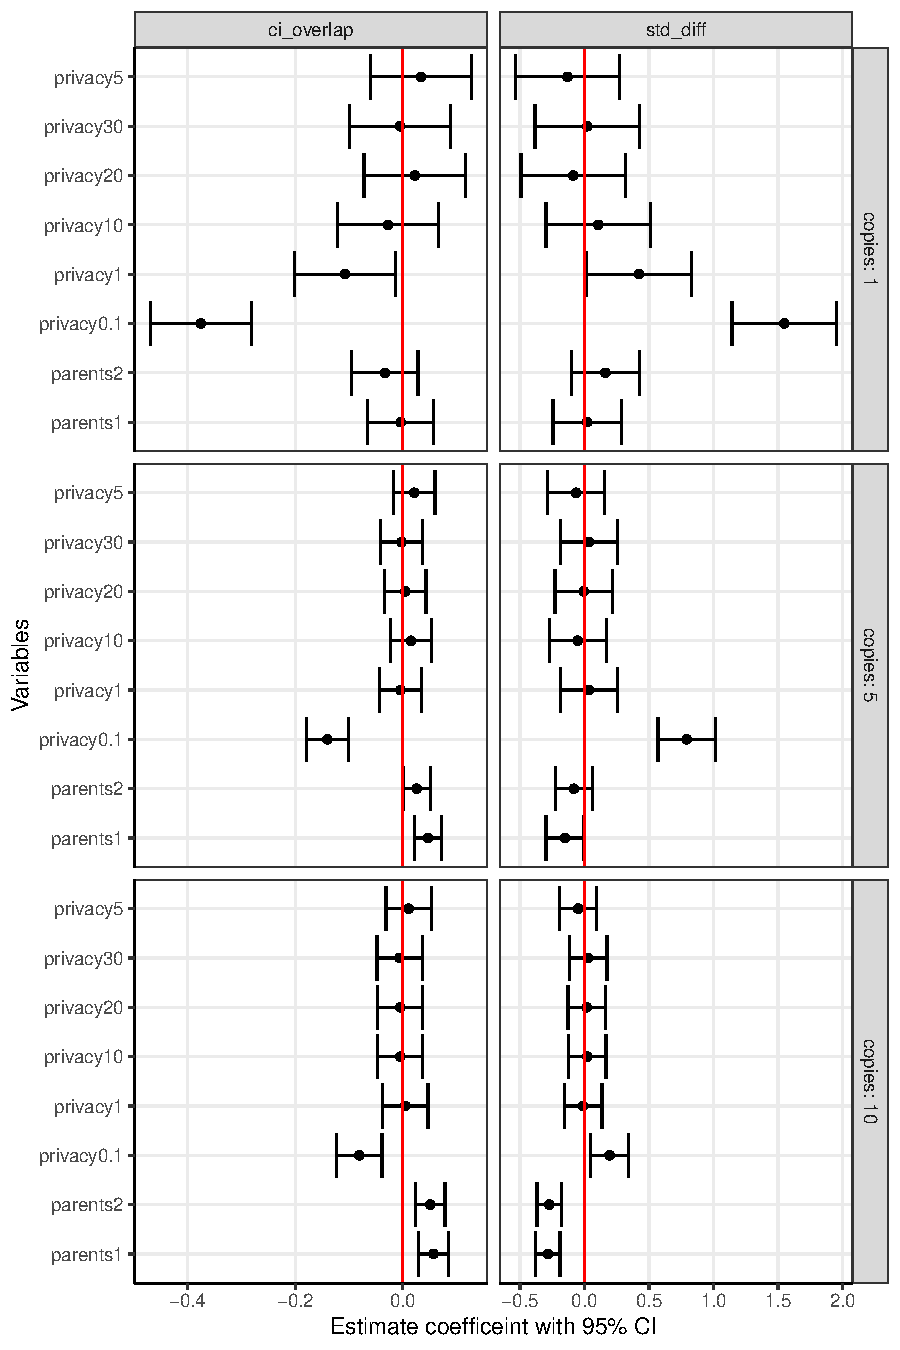
\includegraphics{../graphs/datasynthesizer/graph_datasynthesizer_cio_facet.pdf}
    \label{graph_datasynthesizer_cio_facet}
\end{figure}


\end{document}

